\documentclass[a4]{article}
\pagestyle{myheadings}

%%%%%%%%%%%%%%%%%%%
% Packages/Macros %
%%%%%%%%%%%%%%%%%%%
\usepackage{mathrsfs}



\usepackage{fancyhdr}
\pagestyle{fancy}
\lhead{}
\chead{}
\rhead{}
\lfoot{}
\cfoot{} 
\rfoot{\normalsize\thepage}
\renewcommand{\headrulewidth}{0pt}
\renewcommand{\footrulewidth}{0pt}
\newcommand{\RomanNumeralCaps}[1]
    {\MakeUppercase{\romannumeral #1}}

\usepackage{amssymb,latexsym}  % Standard packages
\usepackage[utf8]{inputenc}
\usepackage[russian]{babel}
\usepackage{MnSymbol}
\usepackage{mathrsfs}
\usepackage{amsmath,amsthm}
\usepackage{indentfirst}
\usepackage{graphicx}%,vmargin}
\usepackage{graphicx}
\graphicspath{{pictures/}} 
\usepackage{verbatim}
\usepackage{color}
\usepackage[nottoc,numbib]{tocbibind}
\usepackage{float}

\usepackage{listings}
\definecolor{codegreen}{rgb}{0,0.6,0}
\definecolor{codegray}{rgb}{0.5,0.5,0.5}
\definecolor{codepurple}{rgb}{0.58,0,0.82}
\definecolor{backcolour}{rgb}{0.95,0.95,0.92}
 
\lstdefinestyle{mystyle}{
    backgroundcolor=\color{backcolour},   
    commentstyle=\color{codegreen},
    keywordstyle=\color{magenta},
    numberstyle=\tiny\color{codegray},
    stringstyle=\color{codepurple},
    basicstyle=\footnotesize,
    breakatwhitespace=false,         
    breaklines=true,                 
    captionpos=b,                    
    keepspaces=true,                 
    numbers=left,                    
    numbersep=5pt,                  
    showspaces=false,                
    showstringspaces=false,
    showtabs=false,                  
    tabsize=2
}
 
\lstset{style=mystyle}

\usepackage{url}
\urldef\myurl\url{foo%.com}





\DeclareGraphicsExtensions{.pdf,.png,.jpg}% -- настройка картинок

\usepackage{epigraph} %%% to make inspirational quotes.
\usepackage[all]{xy} %for XyPic'a
\usepackage{color} 
\usepackage{amscd} %для коммутативных диграмм
%\usepackage[colorlinks,urlcolor=red]{hyperref}

%\renewcommand{\baselinestretch}{1.5}
%\sloppy
%\usepackage{listings}
%\lstset{numbers=left}
%\setmarginsrb{2cm}{1.5cm}{1cm}{1.5cm}{0pt}{0mm}{0pt}{13mm}


\newtheorem{Lemma}{Лемма}[section]
\newtheorem{Proposition}{Предложение}[section]
\newtheorem{Theorem}{Теорема}[section]
\newtheorem{Corollary}{Следствие}[section]
\newtheorem{Remark}{Замечание}[section]
\newtheorem{Definition}{Определение}[section]
\newtheorem{Designations}{Обозначение}[section]




%%%%%%%%%%%%%%%%%%%%%%% 
%Подготовка оглавления% 
%%%%%%%%%%%%%%%%%%%%%%% 
\usepackage[titles]{tocloft}
\renewcommand{\cftdotsep}{2} %частота точек
\renewcommand\cftsecleader{\cftdotfill{\cftdotsep}}
\renewcommand{\cfttoctitlefont}{\hspace{0.38\textwidth} \LARGE\bfseries} 
\renewcommand{\cftsecaftersnum}{.}
\renewcommand{\cftsubsecaftersnum}{.}
\renewcommand{\cftbeforetoctitleskip}{-1em} 
\renewcommand{\cftaftertoctitle}{\mbox{}\hfill \\ \mbox{}\hfill{\footnotesize Стр.}\vspace{-0.5em}} 
%\renewcommand{\cftchapfont}{\normalsize\bfseries \MakeUppercase{\chaptername} } 
%\renewcommand{\cftsecfont}{\hspace{1pt}} 
\renewcommand{\cftsubsecfont}{\hspace{1pt}} 
%\renewcommand{\cftbeforechapskip}{1em} 
\renewcommand{\cftparskip}{3mm} %определяет величину отступа в оглавлении
\setcounter{tocdepth}{5} 
\renewcommand{\listoffigures}{\begingroup %добавляем номер в список иллюстраций
\tocsection
\tocfile{\listfigurename}{lof}
\endgroup}
\renewcommand{\listoftables}{\begingroup %добавляем номер в список иллюстраций
\tocsection
\tocfile{\listtablename}{lot}
\endgroup}


   
   
%\renewcommand{\thelikesection}{(\roman{likesection})}
%%%%%%%%%%%
% Margins %
%%%%%%%%%%%
\addtolength{\textwidth}{0.7in}
\textheight=630pt
\addtolength{\evensidemargin}{-0.4in}
\addtolength{\oddsidemargin}{-0.4in}
\addtolength{\topmargin}{-0.4in}

%%%%%%%%%%%%%%%%%%%%%%%%%%%%%%%%%%%
%%%%%%Переопределение chapter%%%%%% 
%%%%%%%%%%%%%%%%%%%%%%%%%%%%%%%%%%%
\newcommand{\empline}{\mbox{}\newline} 
\newcommand{\likechapterheading}[1]{ 
\begin{center} 
\textbf{\MakeUppercase{#1}} 
\end{center} 
\empline} 

%%%%%%%Запиливание переопределённого chapter в оглавление%%%%%% 
\makeatletter 
\renewcommand{\@dotsep}{2} 
\newcommand{\l@likechapter}[2]{{\bfseries\@dottedtocline{0}{0pt}{0pt}{#1}{#2}}} 
\makeatother 
\newcommand{\likechapter}[1]{ 
\likechapterheading{#1} 
\addcontentsline{toc}{likechapter}{\MakeUppercase{#1}}} 




\usepackage{xcolor}
\usepackage{hyperref}
\definecolor{linkcolor}{HTML}{000000} % цвет ссылок
\definecolor{urlcolor}{HTML}{AA1622} % цвет гиперссылок
 
\hypersetup{pdfstartview=FitH,  linkcolor=linkcolor,urlcolor=urlcolor, colorlinks=true}

%%%%%%%%%%%%
% Document %
%%%%%%%%%%%%

%%%%%%%%%%%%%%%%%%%%%%%%%%%%%
%%%%%%главы -- section*%%%%%%
%%%%section -- subsection%%%%
%subsection -- subsubsection%
%%%%%%%%%%%%%%%%%%%%%%%%%%%%%
\def \newstr {\medskip \par \noindent} 



\begin{document}
\def\contentsname{\LARGE{Содержание}}
\thispagestyle{empty}
\begin{center} 
\vspace{2cm} 
{\Large \sc Санкт-Петербургский Политехнический}\\
\vspace{2mm}
{\Large \sc Университет} им. {\Large\sc Петра Великого}\\
\vspace{1cm}
{\large \sc Институт прикладной математики и механики\\ 
\vspace{0.5mm}
\textsc{}}\\ 
\vspace{0.5mm}
{\large\sc Кафедра прикладной математики}\\
\vspace{15mm}
%\rule[0.5ex]{\linewidth}{2pt}\vspace*{-\baselineskip}\vspace*{3.2pt} 
%\rule[0.5ex]{\linewidth}{1pt}\\[\baselineskip] 
{\huge \sc Лабораторная работа №$3$\\
\vspace{4mm}
Построение разбиения области\\
\vspace{4mm}
между замкнутыми кривыми
\vspace{6mm}
 }
\vspace*{2mm}
%\rule[0.7ex]{\linewidth}{1pt}\vspace*{-\baselineskip}\vspace{3.2pt} 
%\rule[0.5ex]{\linewidth}{2pt}\\ 
\vspace{1cm}

{\sc $4$ курс$,$ группа $3630102/60201$}

\vspace{2cm} 
Студент \hfill Д. А. Плаксин\\
\vspace{1cm}
Преподаватель \hfill Баженов А. Н.\\
\vspace{20mm} 

\end{center} 
%\author{Я}
\begin{center}
\vfill {\large\textsc{Санкт-Петербург}}\\ 
2019 г.
\end{center}

%%%%%%%%%%%%%%%%%%%%%%%%%%%%%%%%%%%%%%%%%%%%%%%%%%%%%%%%%%%%%%%%%%%%%%%%%%%%%%%%%%%%%%%%%%%%%%
%\ \\[4cm]

%\rm
%%%%%%%%%%%%%%%%%%%%%%%%%%%%%%%%%%%%%%%%%%%%%%%%%%%%%%%%%%%%%%%%%%%%%%%%%%%%%%%%%%%%%%%%%%%%%%
\newpage
\pagestyle{plain}

%\begin{center}
%\begin{abstract} 

%\end{abstract}

%\end{center}
\newpage
\tableofcontents{}
\newpage
\listoffigures{}
\newpage

\section{Постановка задачи}
\begin{itemize}
    \item Считать данные из g-файла.

\item Вычислить магнитную ось.

\item Построить кривую сепаратрисы, отметить на графике магнитную ось.

\item Вычислить радиусы кривизны в каждой точке сепаратрисы.

\item Применить к полученным результатам медианно сглаживание.

\item Построить разбиение области сепаратрисы на сетку.
\end{itemize}


\section{Теория}
Сепаратрисы $\--$ граница плазмы, последняя замкнутая поверхность магнитного потока.

Магнитная ось $\--$ экстремум магнитного потока.
\subsection{Радиус кривизны}
По теореме синусов:
\begin{equation}
    \frac{\vert a\vert}{\sin(C)}=2R
\end{equation}

Из скалярного произведения вычислим косинус угла: 
\begin{equation}
    \cos(C)=\frac{(b,c)}{\vert b\vert \vert c\vert}
\end{equation}

Тогда 
\begin{equation}
    \sin(C)=\frac{\vert a\vert}{2\sin(C)}
\end{equation}

\subsection{Построение разбиения сетки}
\begin{itemize}
    \item Делим область на 2 сектора (по экватору)

\item В каждом секторе находим точку с максимальным радиусом кривизны

\item Найдены 4 особые точки (2 на экваторе, 2 в точках с максимальным радиусом кривизны)

\item Внутри каждого сектора проводим ещё N дополнительных отрезков. Итого получено 4N отрезка

\item Находим у каждого из отрезков середину и соединяем их между собой

\item В итоге получили разбиение пространства (сетку)
\end{itemize}

\section{Реализация}
Все задания были выполнены на языке программирования $Matlab$ в среде разработки $MATLAB R2014b$ \hfill \cite{1}

Данные из фала считаны функцией "gfile\_extractor\_1t" \hfill\cite{2}

Радиус кривизны вычислялся по $3$ точкам (как радиус окружности, описанной вокруг треугольника)

$R(i)$ вычисляется по трём точкам: $A = p(i-1), B = p(i), C = p(i+1),$ где $p\;\--$ точки сепаратрисы

Для крайних точек сепаратрисы учитывается её замкнутость


\section{Результаты}

\begin{figure}[H]
\begin{center}
\caption{Радиус кривизны }
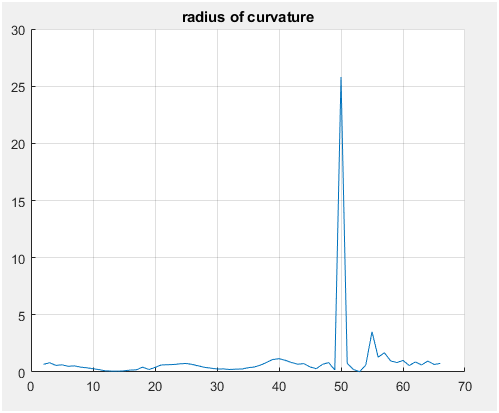
\includegraphics{pic1.png} 

\caption{Радиус кривизны после медианного сглаживания}
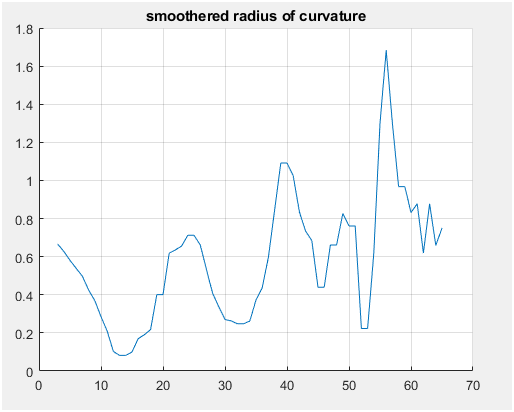
\includegraphics{pic2.png} 
\end{center}
\end{figure}


\begin{figure}[H]
\begin{center}
\caption{Разбиение сетки для сепаратрисы}
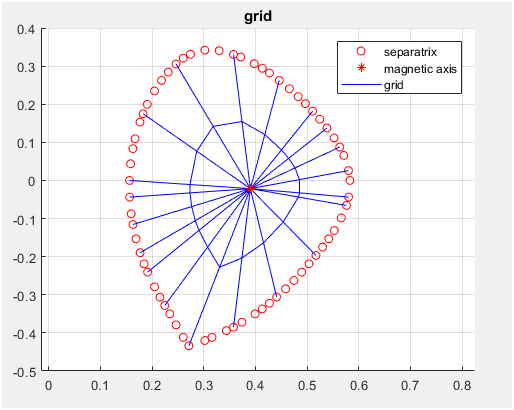
\includegraphics{pic3.png} 
\end{center}
\end{figure}



\section{Обсуждение}
После медианного сглаживания «пики» и «впадины» радиуса кривизны стали более отчетливые.

\begin{thebibliography}{}
    \bibitem{1}  Документация по Матлаб: https://www.mathworks.com/help/ (дата обращения октябрь 2019)

    \bibitem{2} Код функции g\_file\_extractor\_1t: https://cloud.mail.ru/public/5o3T/4G4dD71hL (дата обращения сентябрь 2019)
    
    \bibitem{source}
    Пособие к Лабораторным работам https://cloud.mail.ru/public/4ra6/5wwqBzMBC/LabPractics.pdf
\end{thebibliography}

\section{Приложения}

Код отчёта:\; \url{https://github.com/MisterProper9000/computing-complex/tree/Lab-3-separatrix/Lab_3(separatrix)/texReport/lab3.tex}

Код лаборатрной:\; \url{https://github.com/MisterProper9000/computing-complex/tree/Lab-3-separatrix/Lab_3(separatrix)/texReport/Lab3.m}

\lstinputlisting[language=Matlab]{lab3.m}

\end{document}